\documentclass[12pt,a4paper]{report}
\usepackage[utf8]{inputenc}
\usepackage{amsfonts}
\usepackage{setspace}
\usepackage{graphicx}
\usepackage{array}
\usepackage{fancyhdr}
\usepackage{geometry}
\usepackage{ragged2e}
\usepackage{color}
\usepackage{biblatex}
\usepackage{tabularx}
\usepackage{listings}
\usepackage{xcolor} 


\lstdefinelanguage{JavaScript}{
  keywords={break, case, catch, class, const, continue, debugger, default, delete, do, else, export, extends, false, finally, for, function, if, import, in, instanceof, let, new, null, return, super, switch, this, throw, true, try, typeof, var, void, while, with, yield},
  keywordstyle=\color{blue},
  stringstyle=\color{red},
  commentstyle=\color{green},
  morecomment=[l][\color{magenta}]{//},
  morecomment=[s][\color{magenta}]{/*}{*/},
  morestring=[b]',
  morestring=[b]"
}

\lstset{
  backgroundcolor=\color{lightgray},
  basicstyle=\ttfamily\small,
  keywordstyle=\color{blue},
  commentstyle=\color{green},
  stringstyle=\color{red},
  numbers=left,
  numberstyle=\tiny\color{gray},
  stepnumber=1,
  numbersep=5pt,
  showspaces=false,
  showstringspaces=false,
  showtabs=false,
  frame=single,
  tabsize=2,
  captionpos=b,
  language=JavaScript,  % Set default language to JavaScript
}


\addbibresource{reference.bib}

\geometry{
a4paper,
total={210mm,297mm},
left=1.15in,
right=0.85in,
top=1.0in,
bottom=1.0in,
}

\begin{document}

\pagestyle{empty}

%%%%%%%%%%%%%%%%%%% Front Page  %%%%%%%%%%%%%%%%%%%%%%%
\begin{center}
{\large \textbf{Visvesvaraya Technological University, Belagavi – 590018}}
\begin{figure}[hbtp]
\centering

\includegraphics[width=2.3cm,height=3cm]{./pic/vtu}
\end{figure}

\textbf{MINI-PROJECT REPORT}
\par
\textbf{ON}
\par
\vspace{6pt}
{\Large \textbf{B-LOCK: Blockchain based eVault application}}
\par
\vspace{12pt}
\par
\textit{\textbf{Submitted in partial fulfillment for the award of degree of}}
\par
\vspace{12pt}
\large \textbf{BACHELOR OF ENGINEERING }
\par
\textbf{in}
\par
\large \textbf{COMPUTER SCIENCE \& ENGINEERING}
\par
\vspace{12pt}
\textit{\textbf{Submitted by}}

\begin{center}
\begin{tabular}{l@{\hspace{2cm}}r}
\textbf{\large Abhik L Salian } & \textbf{4SO21CS004} \\
\textbf{\large Ashwitha Shetty} & \textbf{4SO21CS030} \\
\textbf{\large H Karthik P Nayak } & \textbf{4SO21CS058} \\
\textbf{\large Jessica Lillian Mathew } & \textbf{4SO21CS066} \\
\end{tabular}
\end{center}

\vspace{12pt}
\textit{\textbf{Under the Guidance of}}
\par
\vspace{6pt}
\textbf{Dr. Santhosh Kumar DK}
\par
\vspace{2pt}
\normalsize {Associate Professor, Department of CSE}
\par
\begin{figure}[hbtp]
\centering

\includegraphics[scale=0.6]{./pic/sjeclogo}
\end{figure}
\large \textbf{DEPT. OF COMPUTER SCIENCE AND ENGINEERING}
\par \Large \textbf{ST JOSEPH ENGINEERING COLLEGE}
\par 
\textbf{An Autonomous Institution}
\par
{\large{(Affiliated to VTU Belagavi, Recognized by AICTE, Accredited by NBA)}}
\par
{\large \textbf{Vamanjoor, Mangaluru - 575028, Karnataka}}
\par 
{\Large \textbf{2023-24}}
\end{center}
\newpage

%%%%%%%%%%%%%%%%%%%%%%%%%% Certificate Page %%%%%%%%%%%%%%%%%%%%%%%%%%%%%%
\begin{center}
\LARGE \textbf{ST JOSEPH ENGINEERING COLLEGE}
\par
\Large \textbf{An Autonomous Institution}
\par \large{(Affiliated to VTU Belagavi, Recognized by AICTE, Accredited by NBA)}
\par \vspace{3pt}
\large \textbf{Vamanjoor, Mangaluru - 575028, Karnataka}
\par \vspace{12pt}  
\par
\large \textbf{DEPT. OF COMPUTER SCIENCE AND ENGINEERING}
\par
\begin{figure}[hbtp]
\centering

\includegraphics[scale=0.5]{./pic/sjeclogo}
\end{figure}


{\Large \textbf{CERTIFICATE}}
\end{center}
\justifying
\par
\setstretch{1.2}
\vspace{0.10in}
\noindent 
Certified that the Mini-project work entitled \textbf{``B-LOCK: Blockchain based eVault application''} carried out by\vspace{2pt} 
\par
\noindent 
\begin{center}
\begin{tabular}{l@{\hspace{2cm}}r}
\textbf{\large Abhik L Salian } & \textbf{4SO21CS004} \\
\textbf{\large Ashwitha Shetty} & \textbf{4SO21CS030} \\
\textbf{\large H Karthik P Nayak } & \textbf{4SO21CS058} \\
\textbf{\large Jessica Lillian Mathew } & \textbf{4SO21CS066} \\
\end{tabular}
\end{center}
\noindent
the bonafide students of VI semester Computer Science \& Engineering in partial fulfillment for the award of Bachelor of Engineering in Computer Science and Engineering of the Visvesvaraya Technological University, Belagavi during the year 2023-2024. It is certified that all suggestions indicated during internal assessment have been incorporated in the report. The project report has been approved as it satisfies the academic requirements in respect of project work prescribed for the said degree. 


\vspace{0.55in}
\par
\vspace{0.65in}
\setstretch{1.15}

\begin{tabularx}{0.95 \textwidth} { 
   >{\raggedright\arraybackslash}X 
   >{\centering\arraybackslash}X 
   >{\raggedleft\arraybackslash}X  }
     \textbf{Ms. L Hema} &  \textbf{Dr Sridevi Saralaya}\\
     Mini-Project Coordinator &   HOD-CSE \\
\end{tabularx}




%%%%%%%%%%%%%%%%%%%%%%%%%% Abstract %%%%%%%%%%%%%%%

\pagestyle{plain}
\setstretch{1.5}
\pagenumbering{roman}
\chapter*{Abstract}
\addcontentsline{toc}{chapter}{\numberline{}Abstract}
The advent of blockchain technology has revolutionized the 
way data is stored and managed, security, transparency, and 
immutability. This report presents the development of a 
blockchain-based eVault, a decentralized 
application designed to securely store, retrieve, download, 
and delete files and documents. The eVault leverages blockchain's 
distributed ledger technology to ensure the integrity and 
confidentiality of users' data.

The primary objective of this project is to provide a robust 
and user-friendly platform for secure document management, 
addressing the increasing demand for data privacy and protection. 
The eVault application allows users to upload files directly 
onto the blockchain, where each document is encrypted and 
assigned a unique identifier for easy retrieval. Users can 
access their documents at any time, with the assurance that 
the data remains untampered due to the immutable nature of 
blockchain records.
 
Key features include secure file upload, efficient retrieval 
using unique identifiers, and comprehensive access control 
mechanisms that ensure data is accessible only to authorized 
users. Performance metrics indicate that the system achieves 
optimal transaction speeds and data retrieval times, even 
under high loads.

Throughout the development process, challenges such as 
scalability and integration with existing systems were 
addressed, resulting in a versatile solution that meets industry 
demands. 

This blockchain-based eVault demonstrates significant potential 
across various industries, offering a secure and efficient 
solution for managing sensitive documents. By addressing current 
limitations in data storage and retrieval, this project paves 
the way for innovative advancements in digital security and 
privacy.

\setstretch{1.2}
\renewcommand{\contentsname}{Table of Contents}
\tableofcontents
\addcontentsline{toc}{chapter}{\numberline{}Table of Contents}
\listoffigures
\addcontentsline{toc}{chapter}{\numberline{}List of Figures}
\listoftables
\addcontentsline{toc}{chapter}{\numberline{}List of Tables}
\newpage

%%%%%%%%%%%%%%%%%%%%% Headers and Footers %%%%%%%%%%%%%%%

\pagestyle{fancy}
\fancyhf{}
\lhead{\fontsize{10}{12} \selectfont B-LOCK: Blockchain based eVault application}
\rhead{\fontsize{10}{12} \selectfont Chapter \thechapter}
\lfoot{\fontsize{10}{12} \selectfont Department of Computer Science and Engineering, SJEC, Mangaluru}
\rfoot{\fontsize{10}{12} \selectfont Page \thepage}
\renewcommand{\headrulewidth}{0.5pt}
\renewcommand{\footrulewidth}{0.5pt}


%%%%%%%%%%%%%%%%%%%%%%% CHapetr 1 Introduction %%%%%%%%%%%%%

\setstretch{1.2}
\pagenumbering{arabic}

\chapter{Introduction}

\section{Background}

In today's digital age, the management and security of data have become paramount across numerous industries. With the rapid increase in data generation, there is a growing need for efficient and secure systems to store, retrieve, and manage sensitive information. Traditional storage solutions often struggle with issues of security breaches, data tampering, and unauthorized access. 

Blockchain technology has emerged as a revolutionary solution to these challenges, offering a decentralized and immutable ledger that enhances data integrity, transparency, and security. By leveraging blockchain, we can ensure that data is stored in a manner that is resistant to tampering and unauthorized access, making it an ideal solution for managing sensitive documents and files.

This report introduces the development of a blockchain-based eVault, a decentralized application designed to provide a secure platform for storing, retrieving, downloading, and deleting files and documents. The eVault utilizes blockchain's unique capabilities to ensure that user data is encrypted, protected, and accessible only to authorized users, addressing the critical need for data privacy and security in various sectors.

The primary goal of this project is to create a user-friendly platform that leverages blockchain technology to offer a robust solution for document management. This platform allows users to securely upload files to the blockchain, ensuring that each document is encrypted and assigned a unique identifier for easy and secure retrieval. The immutable nature of blockchain ensures that once data is stored, it cannot be altered or deleted without proper authorization, providing a high level of trust and reliability.


\section{Problem statement }
In today's digital age, securing sensitive data is a major challenge due to the limitations of traditional storage systems, which often struggle with data breaches, unauthorized access, and tampering. There is an urgent need for a reliable solution that ensures data integrity, privacy, and security. The blockchain-based eVault addresses these issues by providing a decentralized platform for secure file storage, retrieval, download, and deletion, leveraging blockchain technology to guarantee data protection and user control.

\section{Scope}
The blockchain-based eVault project aims to develop a secure and efficient platform for managing sensitive documents across various industries. This project focuses on creating a user-friendly application that allows users to store, access, and manage files with complete confidence in their security.

The eVault will feature encrypted file storage, ensuring that all documents are tamper-proof and accessible only to authorized users. It will implement unique identifiers and access control mechanisms for efficient data retrieval and user management, providing a reliable alternative to conventional storage systems.

The application is particularly suited for sectors where data privacy is critical, such as finance, healthcare, and legal services. By offering a robust solution for secure document management, the eVault project addresses the growing demand for data security and privacy, paving the way for innovative advancements in digital information management.

%---------------------------- Chapter TWO --------------------------

\chapter{Software Requirements Specification}

\section{Introduction}

The purpose of this Software Requirements Specification (SRS) document is to outline the functional and non-functional requirements for the blockchain-based eVault project. The eVault is a decentralized application designed to provide a secure and user-friendly platform for storing, retrieving, downloading, and deleting files using blockchain technology. This document will serve as a guide for the development team and stakeholders, ensuring that all aspects of the system are well-defined and aligned with the project's goals.

This document is structured into two main sections: Functional Requirements and Non-Functional Requirements. The Functional Requirements section describes the core functionalities that the eVault must provide to meet the user's needs. The Non-Functional Requirements section details the quality attributes, performance standards, and other constraints that the system must adhere to for optimal operation.

\section{Functional Requirements}

The functional requirements define the specific behavior and functionalities of the eVault system. These requirements ensure that the application meets user expectations and provides the necessary capabilities for secure document management. The key functional requirements for the eVault include:

\textbf{1. User Registration and Authentication:}
   - The system must allow users to register and create an account using a secure registration process.
   - Users must be able to log in using their credentials, with multi-factor authentication for added security.
   - Passwords must be stored securely using encryption.

\textbf{2. Secure File Upload:}
   - Users must be able to upload files to the eVault, where each file is encrypted before storage.
   - The system must assign a unique identifier to each file for easy retrieval and management.

\textbf{3. File Retrieval and Access Control:}
   - Users must be able to search and retrieve files using the unique identifiers.
   - Access control mechanisms must be implemented to ensure that only authorized users can access specific files.

\textbf{4. File Download and Deletion:}
   - Users must be able to download files securely, with the option to decrypt them upon download.
   - Users should be able to delete files, ensuring that the deletion process is secure and irreversible.

\textbf{5. Blockchain Integration:}
   - The system must integrate with a blockchain platform to ensure the immutability and security of stored files.
   - All transactions related to file operations (upload, download, delete) must be recorded on the blockchain for auditability.

\textbf{6. User Interface:}
   - The application must provide a user-friendly interface that is intuitive and easy to navigate.
   - The interface should support multiple languages and accessibility features.

\section{Non-Functional Requirements}

The non-functional requirements define the quality attributes, performance standards, and other constraints of the eVault system. These requirements ensure that the application operates efficiently and meets user expectations regarding performance, security, and usability. The key non-functional requirements for the eVault include:

\textbf{1. Performance:}
   - The system must handle a high volume of transactions and file uploads/downloads without significant delays.
   - File retrieval times should not exceed a specified threshold, ensuring quick access to documents.

\textbf{2. Scalability:}
   - The eVault must be able to scale to accommodate a growing number of users and files.
   - The system should support horizontal scaling to handle increased demand.

\textbf{3. Security:}
   - All data, including user credentials and files, must be encrypted to protect against unauthorized access and breaches.
   - The system should comply with industry security standards and regulations (e.g., GDPR, HIPAA).

\textbf{4. Reliability:}
   - The eVault must provide high availability and uptime, minimizing downtime and disruptions.
   - The system should have backup and recovery mechanisms to ensure data integrity and availability.

\textbf{5. Usability:}
   - The application should be intuitive and easy to use, with clear instructions and help resources available.
   - User feedback mechanisms should be in place to gather input for future improvements.

\textbf{6. Compatibility:}
   - The eVault must be compatible with various operating systems and devices, including desktops, tablets, and smartphones.
   - The system should support major web browsers and adhere to web standards.

\textbf{7. Maintainability:}
   - The system architecture should be modular and easy to maintain, allowing for future updates and enhancements.
   - Code documentation and best practices should be followed to facilitate development and troubleshooting.

   \section{User Interface Requirements}

   This section outlines the design and functional requirements of the user interface (UI) for the eVault system. It includes considerations for usability, accessibility, and aesthetic appeal, ensuring an intuitive experience for all users.
   
   \subsection{Design Principles}
   The user interface should adhere to modern design principles to enhance usability and user satisfaction.
   \begin{itemize}
       \item \textbf{Consistency:} The UI should maintain consistency in design elements across all screens, including fonts, colors, and button styles.
       \item \textbf{Simplicity:} The design should be clean and clutter-free, emphasizing essential functions to avoid overwhelming the user.
       \item \textbf{Clarity:} The interface should be organized in a way that makes it easy for users to navigate and find features. Key actions such as file upload, download, and account management should be easily accessible.
   \end{itemize}
   
   \subsection{Accessibility}
   The application should be accessible to all users, including those with disabilities, by adhering to accessibility standards.
   \begin{itemize}
       \item \textbf{Screen Readers:} The UI should support screen readers to assist visually impaired users in navigating the application.
       \item \textbf{Keyboard Navigation:} Users should be able to navigate the application using keyboard shortcuts without relying on a mouse.
       \item \textbf{Color Contrast:} Ensure sufficient contrast between text and background colors to improve readability for users with visual impairments.
   \end{itemize}
   
   \subsection{User Feedback}
   Feedback mechanisms should be implemented to gather user input and improve the application over time.
   \begin{itemize}
       \item \textbf{Error Messages:} Provide clear and informative error messages to guide users in resolving issues.
       \item \textbf{User Surveys:} Periodic surveys can be conducted to collect user feedback on the UI and identify areas for improvement.
       \item \textbf{Help Resources:} Offer tutorials and help sections to assist users in understanding and using the application's features.
   \end{itemize}
   
   \section{Software Requirements}
   
   This section specifies the technical requirements of the eVault system, covering hardware, software, network, and operational aspects to ensure efficient and reliable performance.
   
   \subsection{Hardware Requirements}
   The eVault system requires specific hardware configurations to operate efficiently and support user needs.
   \begin{itemize}
       \item \textbf{Server Specifications:} Minimum server requirements include 16 GB RAM, 4-core CPU, and 500 GB SSD for optimal performance.
       \item \textbf{User Devices:} Users should have access to devices with at least 4 GB RAM and a modern web browser to use the application effectively.
   \end{itemize}
   
   \subsection{Software Dependencies}
   The eVault relies on various software components and libraries to function correctly.
   \begin{itemize}
       \item \textbf{Operating Systems:} Compatible with Windows, macOS, and Linux for server deployments.
       \item \textbf{Database Systems:} Supports MySQL and MongoDB for data storage and management.
       \item \textbf{Programming Languages:} Developed using Python and JavaScript, leveraging frameworks such as Django and React.
   \end{itemize}
   
   \subsection{Network Requirements}
   Ensure stable and secure network connectivity to support application operations and data transmission.
   \begin{itemize}
       \item \textbf{Bandwidth:} The application requires a minimum internet speed of 10 Mbps for smooth operation.
       \item \textbf{Firewall Settings:} Configure firewalls to allow traffic through necessary ports while blocking unauthorized access.
       \item \textbf{Data Encryption:} All data transmitted over the network must be encrypted using TLS to prevent interception.
   \end{itemize}





\chapter{System Design}
\section{Architecture Design}
\begin{figure}[hbtp]
\centering
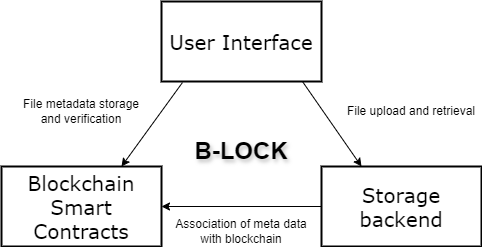
\includegraphics[width=5.5in,height=3in]{./pic/architecture.drawio.png}
\caption{System Architecture Diagram}
\label{fig:architecture}
\end{figure}
Figure \ref{fig:architecture} illustrates the high-level architecture of the B-LOCK system. This architecture comprises several key components: the user interface, blockchain smart contracts, and the storage backend. The user interface allows users to interact with the application, facilitating file uploads and retrieval. The blockchain smart contracts, deployed on Ethereum, handle file metadata storage and verification. The storage backend, implemented using Firebase, manages the actual file storage and retrieval. This design ensures a secure and user-friendly application where file integrity and ownership are maintained through blockchain technology.
\section{Decomposition Description}
\begin{figure}[hbtp]
\centering
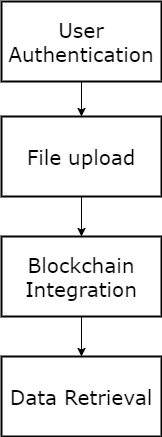
\includegraphics[width=1.7in,height=4in]{./pic/flowchart.png}
\caption{Flow chart}
\label{fig:flowchart}
\end{figure}
Figure \ref{fig:flowchart} presents a decomposition diagram (or a flow chart) of the B-LOCK system. This diagram breaks down the system into its core modules: user authentication, file upload, blockchain integration, and data retrieval. Each module is responsible for specific functionalities:
\begin{itemize}
   \item \textbf{User Authentication:} Manages user sign-in and sign-up, including email verification and session management.
   \item \textbf{File Upload:} Handles file selection, uploading to Firebase Storage, and associating file metadata with the blockchain.
   \item \textbf{Blockchain Integration:} Interacts with Ethereum smart contracts to store and retrieve file hashes and metadata.
   \item \textbf{Data Retrieval:} Provides mechanisms for users to access their uploaded files and associated data.
\end{itemize}


\section{Data Flow Design}

\begin{figure}[hbtp]
\centering
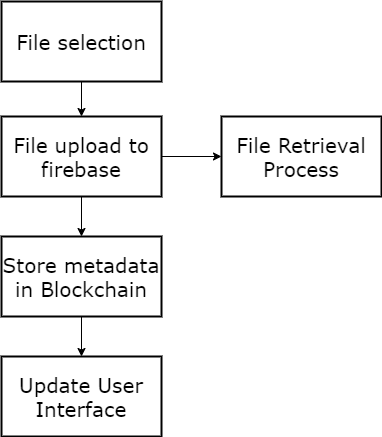
\includegraphics[scale=0.7]{./pic/dataflow.png}
\caption{Dataflow Diagram}
\label{fig:dataflow}
\end{figure}
Figure \ref{fig:dataflow} depicts the data flow within the B-LOCK application. The diagram illustrates the process from file upload to storage and retrieval. When a user uploads a file, the file is first hashed and then uploaded to Firebase Storage. The file's metadata, including its name and hash, is sent to the Ethereum smart contract for secure storage on the blockchain. Upon successful upload, the application updates the user interface to reflect the new file and its status. During file retrieval, the application queries both Firebase and the blockchain to provide users with the necessary information and access to their files.



\chapter{Implementation}
\section{System Overview}
\par
The system is a blockchain-based e-vault application designed to securely store and manage files with metadata. The core components include:
\begin{itemize}
   \item \textbf{Frontend:} A React application for user interaction.
   \item \textbf{Backend:} Firebase for file storage and Firestore for metadata management.
   \item \textbf{Blockchain:} Ethereum for file hash storage and verification.
\end{itemize}

\section{Pseudocode and Algorithms}

\subsection{File Upload Algorithm}

\begin{lstlisting}[caption=File Upload Algorithm]
   function uploadFile(file):
    hash = generateFileHash(file.name, currentTimestamp)
    storageRef = createStorageReference(user.uid, hash, file.name)
    uploadTask = uploadFileToStorage(storageRef, file)

    onUploadProgress(uploadTask):
        progress = calculateUploadProgress(uploadTask)
        displayUploadProgress(progress)

    onUploadComplete(uploadTask):
        downloadURL = getDownloadURL(uploadTask)
        storeFileHashInBlockchain(fileName, fileHash)
        saveFileMetadataInFirestore(fileName, downloadURL, user.uid)
        displaySuccessMessage("File uploaded successfully")

    onUploadError(uploadTask):
        displayErrorMessage("Error uploading file")

   \end{lstlisting}
   
\begin{itemize}
   \item \textbf{Generate File Hash:} Create a unique hash using the file name and current timestamp.
   \item \textbf{Create Storage Reference:} Create a reference in Firebase Storage using the hash and file name.
   \item \textbf{Upload File:} Perform the file upload asynchronously.
   \item \textbf{Progress Monitoring:} Update progress based on the upload state.
   \item \textbf{Completion Handling:} On success, store the file hash in the blockchain and metadata in Firestore.
   \item \textbf{Error Handling:} Display appropriate error messages if the upload fails.
\end{itemize}

\subsection{User Authentication Algorithm}
\begin{lstlisting}[caption=User Authentication Algorithm]
   function signIn(email, password):
    try:
        user = authenticateUserWithEmail(email, password)
        if user.isEmailVerified:
            redirectToDashboard()
        else:
            displayErrorMessage("Email not verified")
    except AuthenticationError as e:
        displayErrorMessage(e.message)
   \end{lstlisting}
\begin{itemize}
   \item \textbf{Authenticate User:} Check user credentials against Firebase Authentication.
   \item \textbf{Email Verification Check:} Ensure the user’s email is verified before granting access.
   \item \textbf{Error Handling:} Handle and display errors during authentication.
\end{itemize}


\section{Key Components Implementation}
\subsection{Frontend (React)}
\par
The frontend is developed using React.js and consists of the following key components:
\begin{itemize}
   \item \textbf{SignIn Component:} Handles user login.
   \item \textbf{SignUp Component:} Manages user registration and email verification.
   \item \textbf{Upload Component:} Manages file upload and progress display.
   \item \textbf{Retrieve Component:} Allows users to view and manage uploaded files.
\end{itemize}
\begin{lstlisting}[caption=Frontend Code Snippet]
   import React, { useState } from 'react';
   import { signInWithEmailAndPassword } from 'firebase/auth';
   import { auth } from './firebase';
   
   const SignIn = ({ onSignIn, switchToSignUp }) => {
       const [email, setEmail] = useState('');
       const [password, setPassword] = useState('');
       const [error, setError] = useState('');
   
       const handleSubmit = async (e) => {
           e.preventDefault();
           try {
               const userCredential = await signInWithEmailAndPassword(auth, email, password);
               const user = userCredential.user;
   
               if (user.emailVerified) {
                   onSignIn(email, password);
                   setError(''); // Clear previous errors
               } else {
                   setError('Please verify your email before signing in.');
                   alert('Email not verified. Please check your inbox for the verification email.');
               }
           } catch (err) {
               console.error("Sign-in error:", err);
               setError(err.message);
           }
       };
   
       return (
           <div className="auth-form">
               <h2>Sign In</h2>
               <form onSubmit={handleSubmit}>
                   <input 
                       type="email" 
                       placeholder="Email" 
                       value={email} 
                       onChange={(e) => setEmail(e.target.value)} 
                       required 
                   />
                   <input 
                       type="password" 
                       placeholder="Password" 
                       value={password} 
                       onChange={(e) => setPassword(e.target.value)} 
                       required 
                   />
                   <button type="submit">Sign In</button>
               </form>
               {error && <p className="error">{error}</p>}
               <p>Don't have an account? <button onClick={switchToSignUp}>Sign Up</button></p>
           </div>
       );
   };
   
   export default SignIn;
   
   \end{lstlisting}

\subsection{Backend (Firebase and Blockchain)}
\begin{itemize}
   \item \textbf{Firebase Storage:} Stores the uploaded files.
   \item \textbf{Firestore Database:} Saves metadata about the files.
   \item \textbf{Ethereum Blockchain:} Stores the file hashes for verification.
\end{itemize}
\begin{lstlisting}[caption=Backend Code Snippet]
   import { ref, uploadBytesResumable, getDownloadURL } from "firebase/storage";
import { collection, addDoc } from "firebase/firestore";

const uploadFile = async (file, user, storage, db, evault, account) => {
    const hash = CryptoJS.SHA256(file.name + new Date().toISOString()).toString();
    const storageRef = ref(storage, `uploads/${user.uid}/${hash}_${file.name}`);
    const uploadTask = uploadBytesResumable(storageRef, file);

    uploadTask.on(
        "state_changed",
        (snapshot) => {
            const progress = (snapshot.bytesTransferred / snapshot.totalBytes) * 100;
            console.log(`Upload is ${progress.toFixed(2)}% done`);
        },
        (error) => {
            console.error("Upload error:", error);
        },
        async () => {
            const downloadURL = await getDownloadURL(uploadTask.snapshot.ref);
            try {
                await evault.methods.storeFile(file.name, hash).send({ from: account });
                await addDoc(collection(db, "files"), {
                    name: file.name,
                    owner: user.uid,
                    downloadURL,
                    timestamp: new Date(),
                });
                console.log("File uploaded successfully");
            } catch (error) {
                console.error("Error saving file data", error);
            }
        }
    );
};

   \end{lstlisting}


\section{Integration}
\par The frontend components interact with the Firebase 
backend and Ethereum blockchain to provide a seamless user 
experience. Authentication is handled via Firebase 
Authentication, ensuring that users are securely signed in. 
File uploads are managed through Firebase Storage, allowing 
users to upload and access their files easily. Metadata related 
to the files, such as names and download URLs, is stored in 
Firestore, providing quick and reliable access to file 
information. The integration with the Ethereum blockchain 
guarantees that file hashes are securely stored and verifiable, 
leveraging smart contracts to maintain the integrity and 
ownership of each file. This combination of Firebase and 
blockchain technologies ensures that the application is both 
secure and scalable, providing a robust solution for digital
 file management.




\chapter{Results and Discussion}
\section{Results}
\par After successfully implementing B-LOCK, our blockchain-based e-vault application, we conducted a series of tests to evaluate its performance and functionality. Below are the key results from these tests:
\begin{enumerate}
   \item User Authentication and Verification:
   \begin{itemize}
      \item \textbf{Result:} The application successfully authenticated users via Firebase Authentication.
      \item \textbf{Discussion:} The integration of Firebase ensured a smooth and secure sign-in process. Users received verification emails promptly, and only verified users could upload and access files.
   \end{itemize}
   \item File Upload and Storage:
   \begin{itemize}
      \item \textbf{Result:} Files were uploaded to Firebase Storage and their metadata was correctly stored in Firestore.
      \item \textbf{Discussion:} Upload speeds were satisfactory, and users were able to retrieve download URLs without delay. The metadata storage in Firestore allowed for efficient file management and retrieval.
   \end{itemize}
   \item Blockchain Integration:
   \begin{itemize}
      \item \textbf{Result:} File hashes were successfully stored on the Ethereum blockchain.
      \item \textbf{Discussion:} Storing file hashes on the blockchain provided an additional layer of security, ensuring the integrity and ownership of files. Users could verify their file's existence and authenticity using blockchain transactions.
   \end{itemize}
   \item Performance Metrics:
   \begin{itemize}
      \item \textbf{Result:} The system handled concurrent uploads and downloads efficiently.
      \item \textbf{Discussion:} The application's performance remained stable under various load conditions. The integration of Firebase and blockchain technologies did not significantly impact the responsiveness of the application.
   \end{itemize}
\end{enumerate}

\section{Discussion}
The development of B-LOCK has shown promising results in creating a secure and reliable e-vault application using blockchain technology. Several key aspects were highlighted during the development and testing phases:
\begin{itemize}
   \item \textbf{Security:} The use of Firebase Authentication provided a robust mechanism for user verification. Combining this with blockchain for storing file hashes enhanced security by ensuring file integrity and ownership, making it difficult for unauthorized users to tamper with the stored data.
   \item \textbf{Scalability:} The architecture of B-LOCK allows for scalability. Firebase’s cloud-based solutions can handle an increasing number of users and files. The use of blockchain, while slightly increasing transaction time due to network confirmations, scales effectively with user demand for verification and integrity checks.
   \item \textbf{User Experience:} User feedback indicated a positive experience with the interface and the ease of use for both uploading and retrieving files. The clear instructions and responsive design contributed to a smooth user journey.
   \item \textbf{Integration Challenges:} Integrating blockchain with traditional cloud services like Firebase posed some challenges, particularly in ensuring seamless interaction between different technologies. However, these were overcome with thorough testing and incremental integration approaches.
\end{itemize}

\section{Screenshots}
Below are screenshots of the B-LOCK application demonstrating key features and user interface elements.

\subsection{User Registration and Login}
\begin{figure}[hbtp]
    \centering
    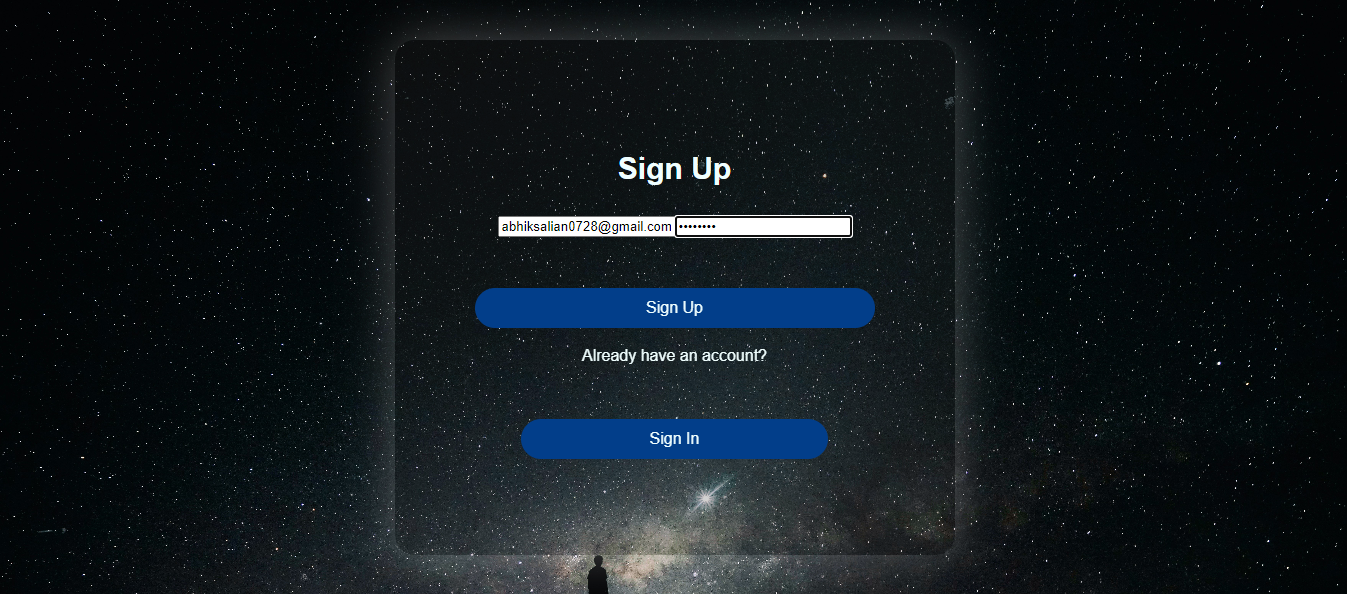
\includegraphics[scale=0.4]{./pic/signup.png}
    \caption{Sign Up Page to register new users}
    \label{fig:signup}
\end{figure}
\begin{figure}[hbtp]
    \centering
    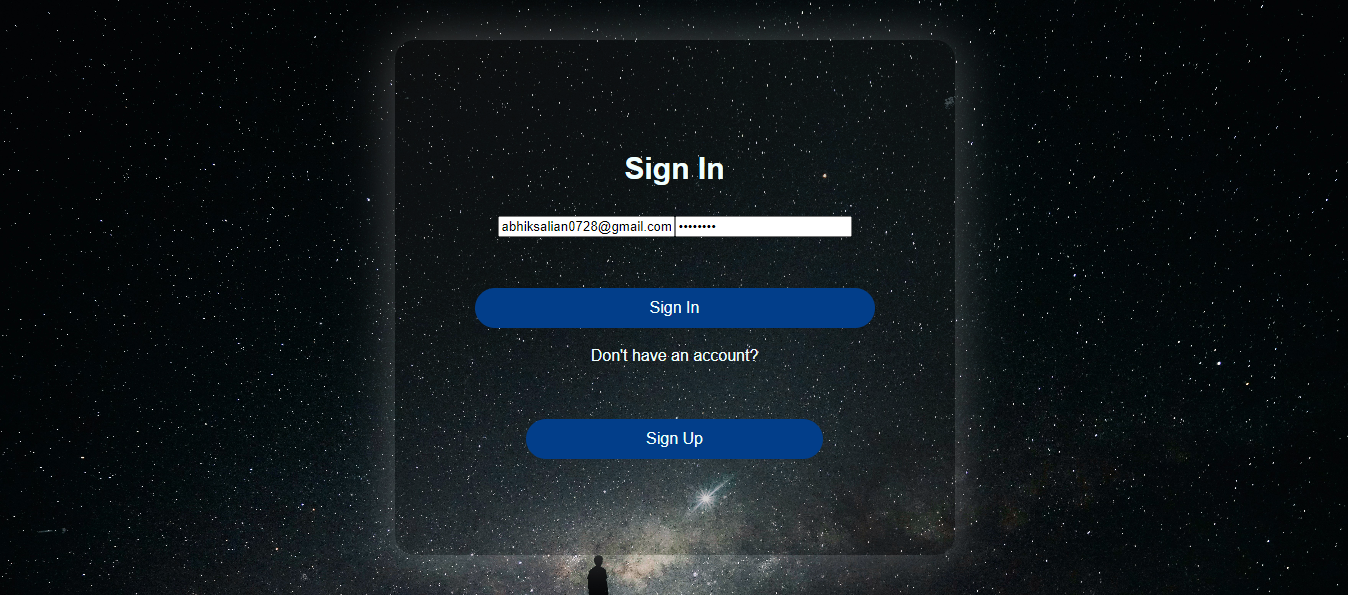
\includegraphics[scale=0.4]{./pic/signin.png}
    \caption{Sign In Page to login already registered users}
    \label{fig:signin}
\end{figure}
\begin{figure}[hbtp]
    \centering
    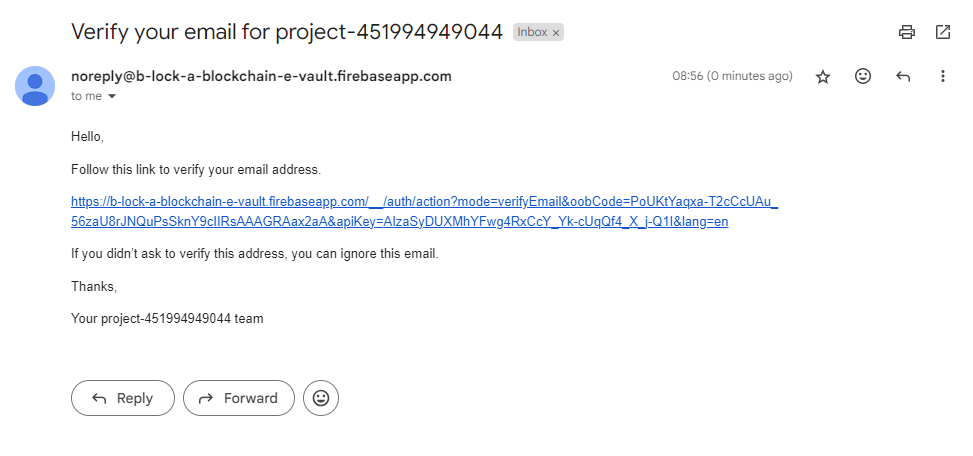
\includegraphics[scale=0.4]{./pic/emailver.png}
    \caption{Verification email that users receive after signing up}
    \label{fig:emailver}
\end{figure}
Figures \ref{fig:signup} and \ref{fig:signin} show the user registration and login interface. Users can create an account by entering their email and password, and existing users can sign in using their credentials. Upon successful registration, a verification email is sent to the user to confirm their email address before accessing the application, as shown in Figure \ref{fig:emailver}.

\subsection{File Upload Interface}
\begin{figure}[hbtp]
    \centering
    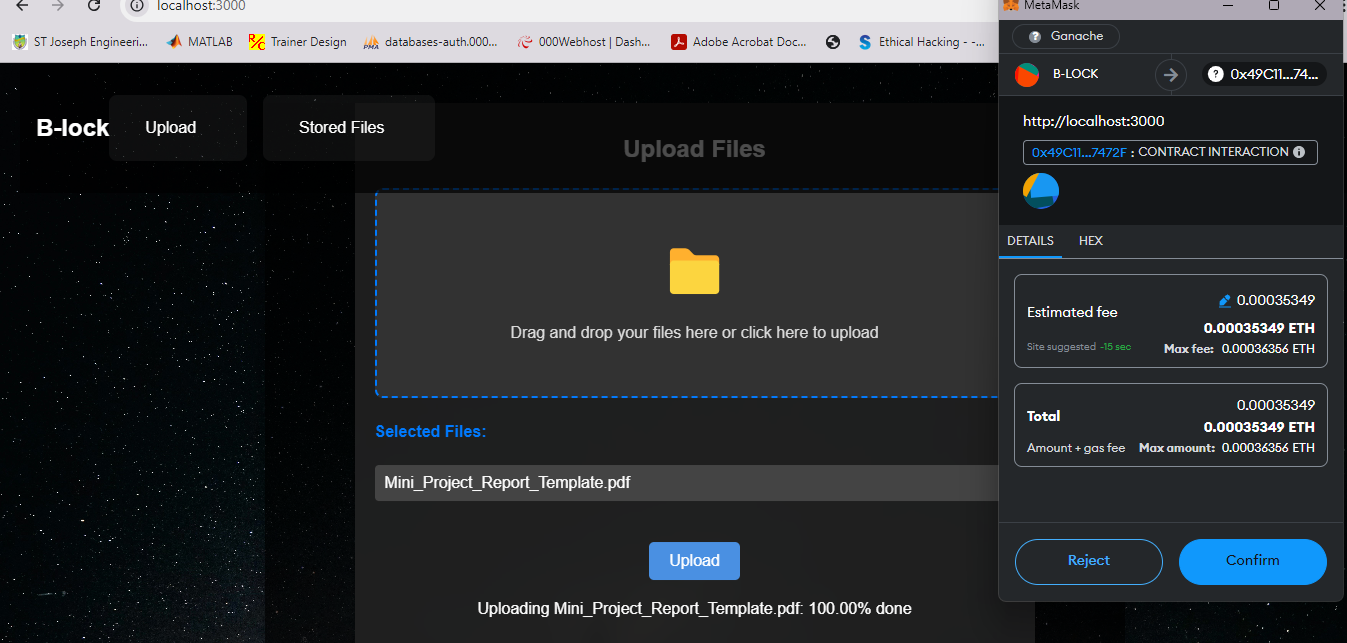
\includegraphics[scale=0.4]{./pic/fileupload.png}
    \caption{File Upload Interface}
    \label{fig:fileupload}
\end{figure}
The file upload interface, as shown in Figure \ref{fig:fileupload}, allows users to select files from their local device to upload to the e-vault. The interface supports multiple file uploads and provides feedback on the upload progress. Users are notified of the upload status, ensuring they are aware of successful uploads or any errors encountered during the process.

\subsection{File Management Dashboard}
\begin{figure}[hbtp]
    \centering
    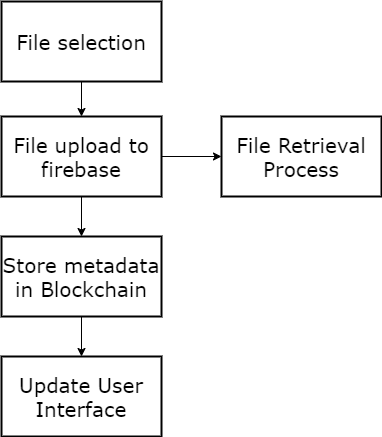
\includegraphics[scale=0.4]{./pic/dataflow.png}
    \caption{File Management Dashboard}
    \label{fig:dashboard}
\end{figure}
Figure \ref{fig:dashboard} displays the file management dashboard, where users can view the list of uploaded files. The dashboard provides details such as the file name, upload date, and file size. Users can also download or delete files from this interface, making it easy to manage their stored documents.

\subsection{File Details and Blockchain Verification}
\begin{figure}[hbtp]
    \centering
    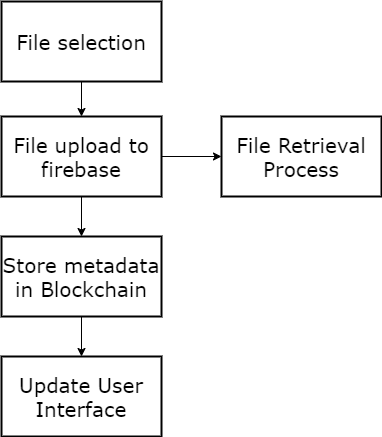
\includegraphics[scale=0.5]{./pic/dataflow.png}
    \caption{File Details and Blockchain Verification}
    \label{fig:filedetails}
\end{figure}
Figure \ref{fig:filedetails} shows the file details page, where users can view specific information about their uploaded files. The page includes the file name, hash, and download link. Additionally, it shows the blockchain verification status, confirming that the file hash has been successfully stored on the Ethereum blockchain, ensuring the integrity and authenticity of the file.


\chapter{Conclusion and Future Work}
\section{Conclusion}
% \cite{bashir2021subjective} \cite{mittal2016}
The B-LOCK project successfully demonstrates the integration of blockchain technology with file storage solutions to create a secure e-vault application. Throughout the development process, we addressed critical aspects of data security, user authentication, and file integrity. By leveraging Ethereum's blockchain, we ensured that every uploaded file is securely hashed and its integrity verifiable, thus preventing unauthorized tampering or data breaches.
\\
Key accomplishments of the B-LOCK project include:
\begin{itemize}
\item \textbf{Secure File Uploads:} Implementation of an intuitive interface allowing users to upload files securely.
\item \textbf{Blockchain Verification:} Integration with the Ethereum blockchain to store file hashes, ensuring the authenticity and integrity of uploaded files.
\item \textbf{User Authentication:} A robust user registration and login system, including email verification for added security.
\item \textbf{Efficient File Management:} A user-friendly dashboard for managing uploaded files, with options to view, download, and delete files.

\end{itemize}

\section{Future Work}
While the current implementation of B-LOCK meets its primary objectives, there are several areas for potential improvement and expansion. Future work could focus on the following aspects:
\begin{itemize}
   \item \textbf{Enhanced Scalability:} As the user base grows, optimizing the system for better scalability will be crucial. This may involve exploring more efficient blockchain solutions or layer-2 scaling techniques.
   \item \textbf{Mobile Application:} Developing a mobile version of B-LOCK to extend accessibility and usability across various devices.
   \item \textbf{Advanced Security Features:} Integrating additional security measures such as multi-factor authentication (MFA), biometric verification, and encryption for stored files.
   \item \textbf{Decentralized Storage Integration:} Exploring decentralized storage solutions such as IPFS (InterPlanetary File System) or Filecoin to further enhance data availability and redundancy.
   \item \textbf{Smart Contract Enhancements:} Improving the smart contract logic to include features like file versioning, access control, and more sophisticated file-sharing mechanisms.
   \item \textbf{User Experience Improvements:} Continuously refining the user interface and experience based on user feedback and emerging best practices in UI/UX design.
   \item \textbf{Automated Backup and Recovery:} Implementing automated backup and disaster recovery solutions to ensure data availability and integrity in case of system failures.
\end{itemize}
By addressing these areas, B-LOCK can evolve into a more comprehensive and versatile e-vault solution, offering enhanced security, scalability, and user experience. The project's success serves as a testament to the potential of blockchain technology in revolutionizing secure data storage and management systems.


% \cite{Tea} This project has a great potential to make a positive impact on communication and security situations. Its continuous improvement will be important to make this impact 
% even greater example for citing and bibtex for journal paper \cite{croitoru2023diffusion}, conference paper \cite{mohamad2015smart}, citing website \cite{knuthwebsite}, citing book \cite{dirac}




\newpage

\pagestyle{plain}
\renewcommand{\bibname}{References}

\addcontentsline{toc}{chapter}{References}

\printbibliography



\end{document}
